\chapter{Trabalho realizado}
\label{chapter:work-done}

\begin{introduction}
    Neste capítulo irei abordar todo o trabalho desenvolvido durante o período de estágio, organizado em três grandes secções. Na primeira secção abordarei o trabalho realizado durante a analise de \textit{APIs} e bibliotecas, incluindo o porque da escolha final de cada uma.A segunda secção visa comentar o trabalho realizado na interface gráfica do projeto \textit{aniposture}. A terceira secção comenta o trabalho desenvolvido no respetivo \textit{backend}.
\end{introduction}

\section{Análise de bibliotecas}\label{sec:analysis}
Durante este estágio, foram-me atribuídas tarefas de análise e pesquisa, com o objetivo de identificar e selecionar as ferramentas mais adequadas que cumprissem os requisitos necessários para o desenvolvimento da aplicação. Foram, assim, realizadas duas grandes análises: a primeira sobre as \textit{APIs} de georreferenciação e a segunda nas \textit{APIs} de visualização gráfica.

\subsection{APIs georreferenciação}
Esta foi uma das primeiras tarefas que foram-me atribuídas durante o estágio. Antes de começar as comparações, foram definidos alguns requisitos fundamentais, nomeadamente a necessidade de \textit{tiles} em satelite, marcadores, bom desempenho com uma elevada quantidade de pontos e desenho de polígonos. Depois de levantados os requisitos, iniciou-se a análise comparativa entre três \textit{APIs} de georreferenciação o mapbox, openlayers e o googlemaps.

Apesar de partilharem a mesma intenção, criação de mapas interativos, as três bibliotecas são consideravelmente diferentes nas suas implementações. 

\subsubsection{\textbf{OpenLayers}}\label{sec:sub_ol}

\textit{Openlayers} é o biblioteca \textit{free e Open Source} que permite a criação de mapas interativos. Disponibiliza recursos como \textit{raster tiles}, camadas vetoriais e marcadores. Por ser \textit{Open Source}, contem vários \textit{addons} criados pela comunidade que permite alargar as suas funcionalidades. Contudo, apresenta uma linha de aprendizado um pouco mais complexa do que outras alternativas e, por padrão, não contêm  nenhum \textit{tile} em satelite. 

\begin{figure}[h!]
    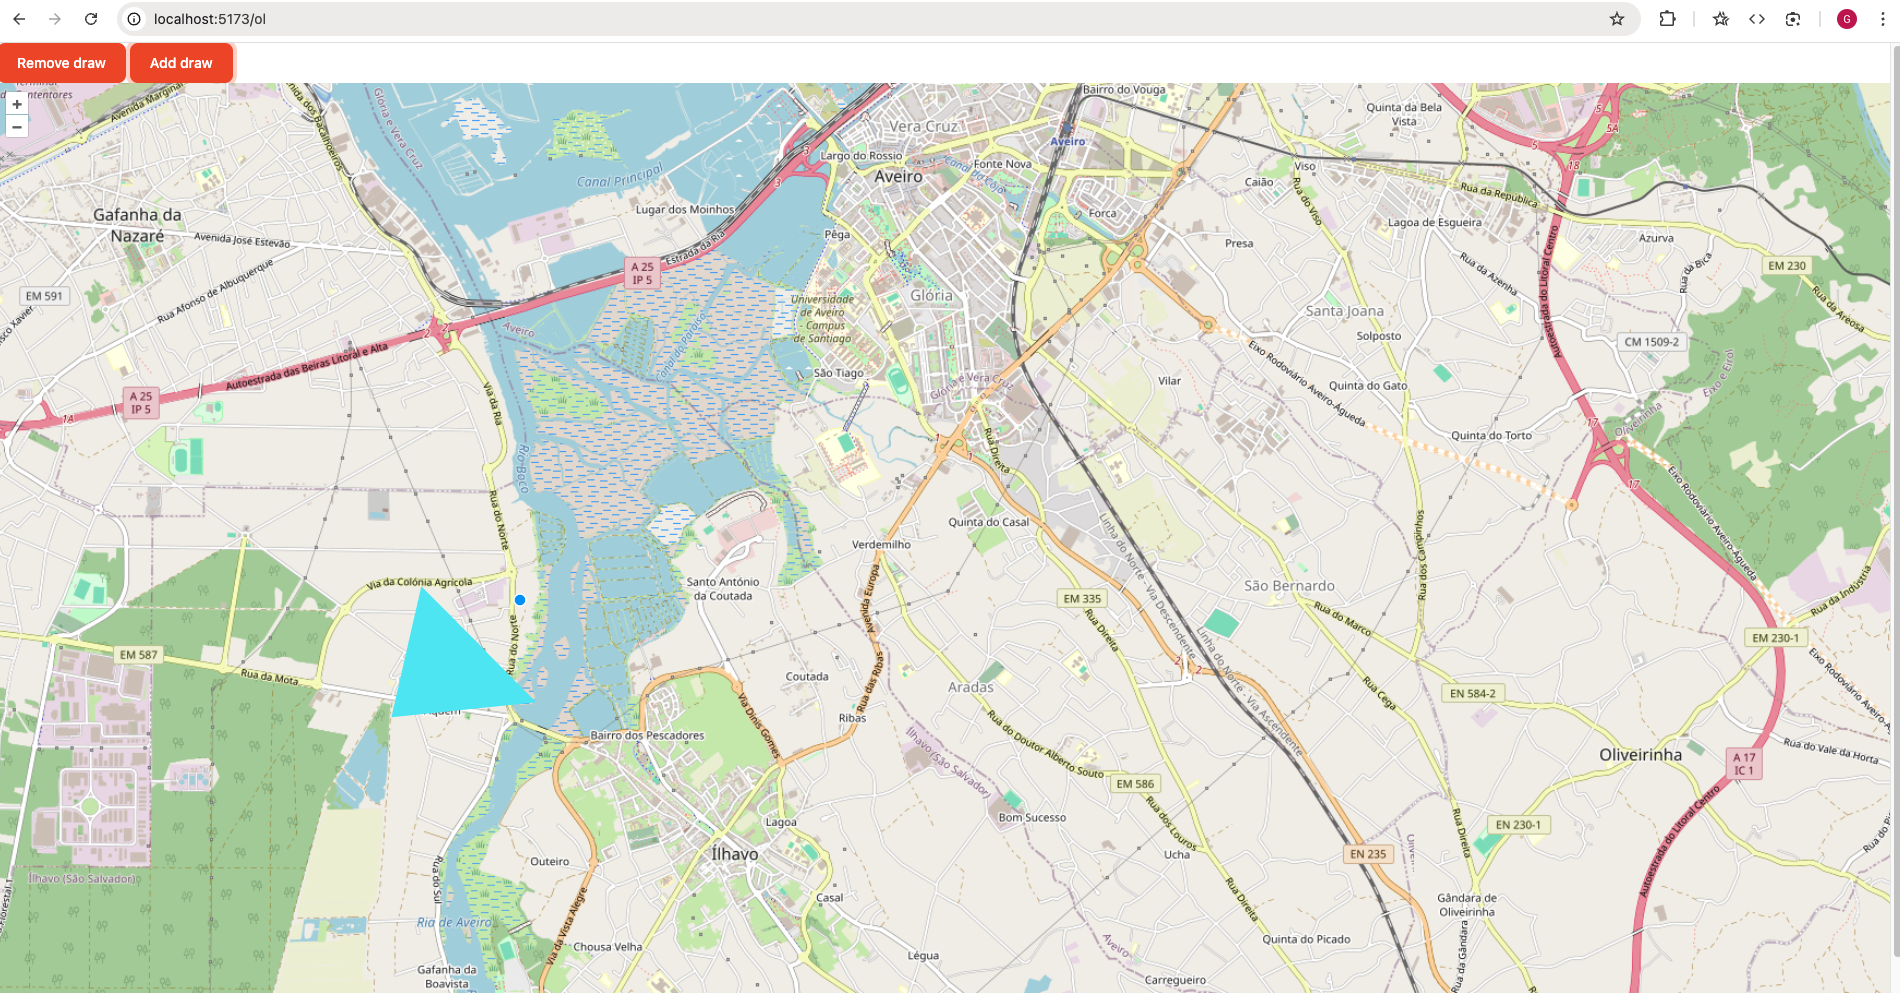
\includegraphics[width=\textwidth]{figs/ol.png}
    \caption[Ol]{OpenLayers}
    \label{fig:ol}
\end{figure}

Foram ainda realizados alguns testes com opções de desenho vetorial. No entanto, o que levou o \textit{OpenLayers} não ser o escolhido foi a sua, ainda, baixa integração com \textit{WebGL}, a documentação menos completa em comparação com outras alternativas e a ausência de suporte nativo para mapa com satélite. 

\subsubsection{\textbf{Google Maps}}\label{sec:sub_gm}
O \textit{google maps} é, muito provavelmente, o sistema de mapas mais utilizado e atualizado a nível mundial. Por essa razão, foi considerada a sua utilização, tendo sido analisada a forma como é implementado e as suas funcionalidades. Inicialmente, esta solução revelou-se a mais promissora, uma vez que permite adicionar camadas vetoriais, marcadores, vista em satélite e um bom desempenho. 

\begin{figure}[h!]
    \centering
    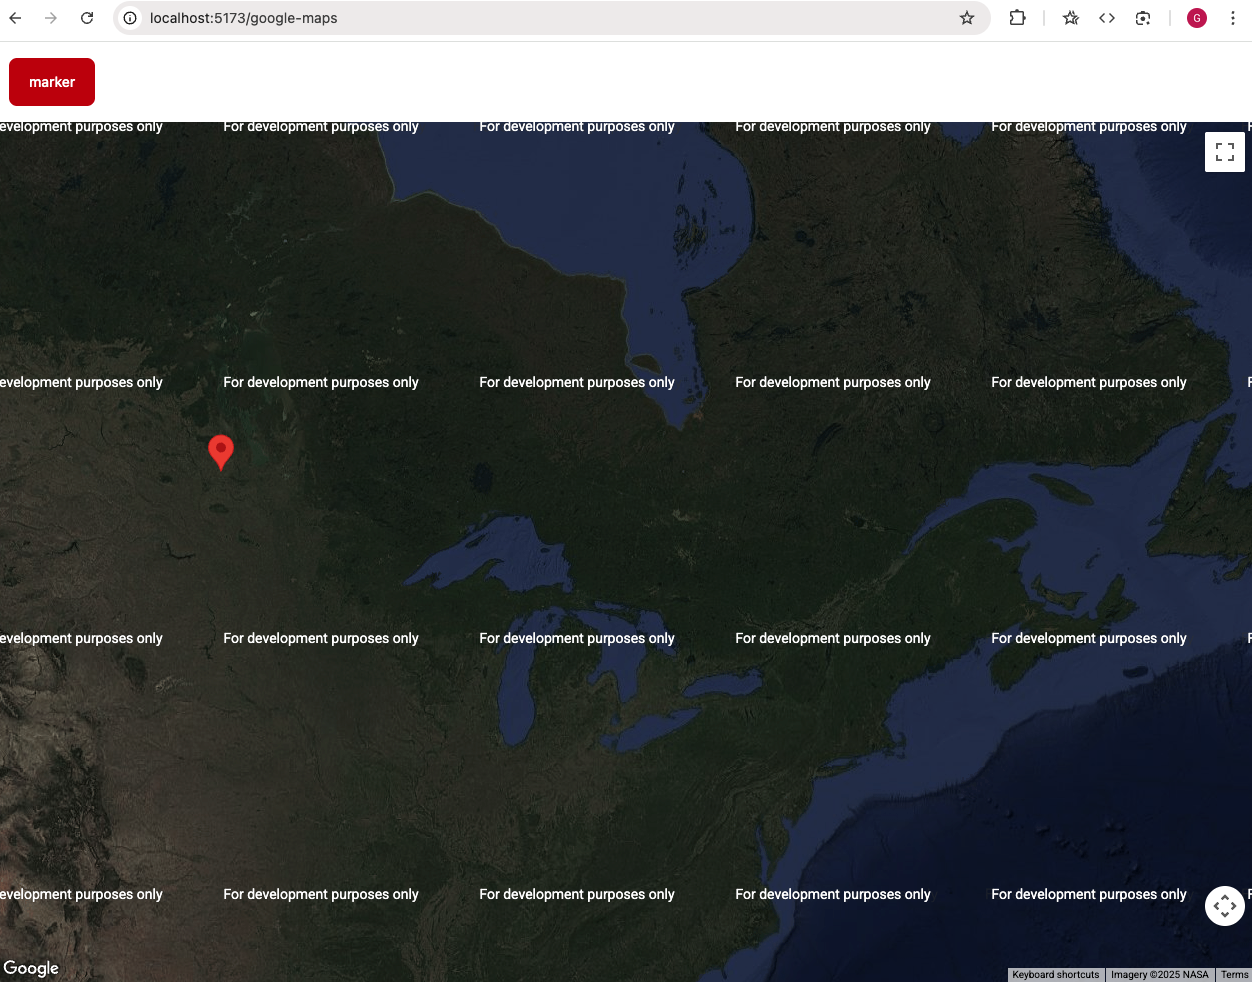
\includegraphics[width=8.95cm]{figs/gm.png}
    \caption[gm]{Google Maps}
    \label{fig:gm}
\end{figure}

Ao contrário do \textit{Openlayers}, \ref{sec:sub_ol}, esta é uma solução paga, que apresenta, algumas vantagens como mapas satélite mais atualizados e integração com os serviços da \textit{Google}. Contudo, o maior problema é o seu preço, consideravelmente elevado se formos comprar com outras alternativas. A \textit{Google} permite a utilização da \href{https://developers.google.com/maps/documentation/javascript}{\textit{Maps JavaScript API}} de forma gratuita até 10.000 pedidos mensais. A partir dessa quantidade começam a ser aplicadas cobranças. Devido a essa limitação o \textit{google maps} também não foi a solução escolhida.

\subsubsection{\textbf{Mapbox}}\label{sec:mapbox}
Chegamos, por fim, à opção escolhida: o \textit{Mapbox}. Esta biblioteca revelou-se a melhor entre os dois mundos, implementação inicial simples, utiliza \textit{WebGL} por padrão e disponibiliza vários tipos de \textit{tiles}, incluindo satélite. Embora seja uma solução paga, apresenta-se modelos mais em conta do que a opção da \textit{google}. Na versão gratuita, contem um total de 50.000 pedidos por mês. Esta mesma quantidade de pedidos no \textit{google maps} teria um custo de cerca de 280€ mensais. Para atingir um custo parecido no \textit{mapbox}, seria necessário utilizar pelo menos 100.000 pedidos mensais. Para além do fator preço/economico, esta solução, compre todos os requisitos definidos para a nossa aplicação, juntamente de uma documentação bem estruturada.

\begin{figure}[h!]
    \centering
    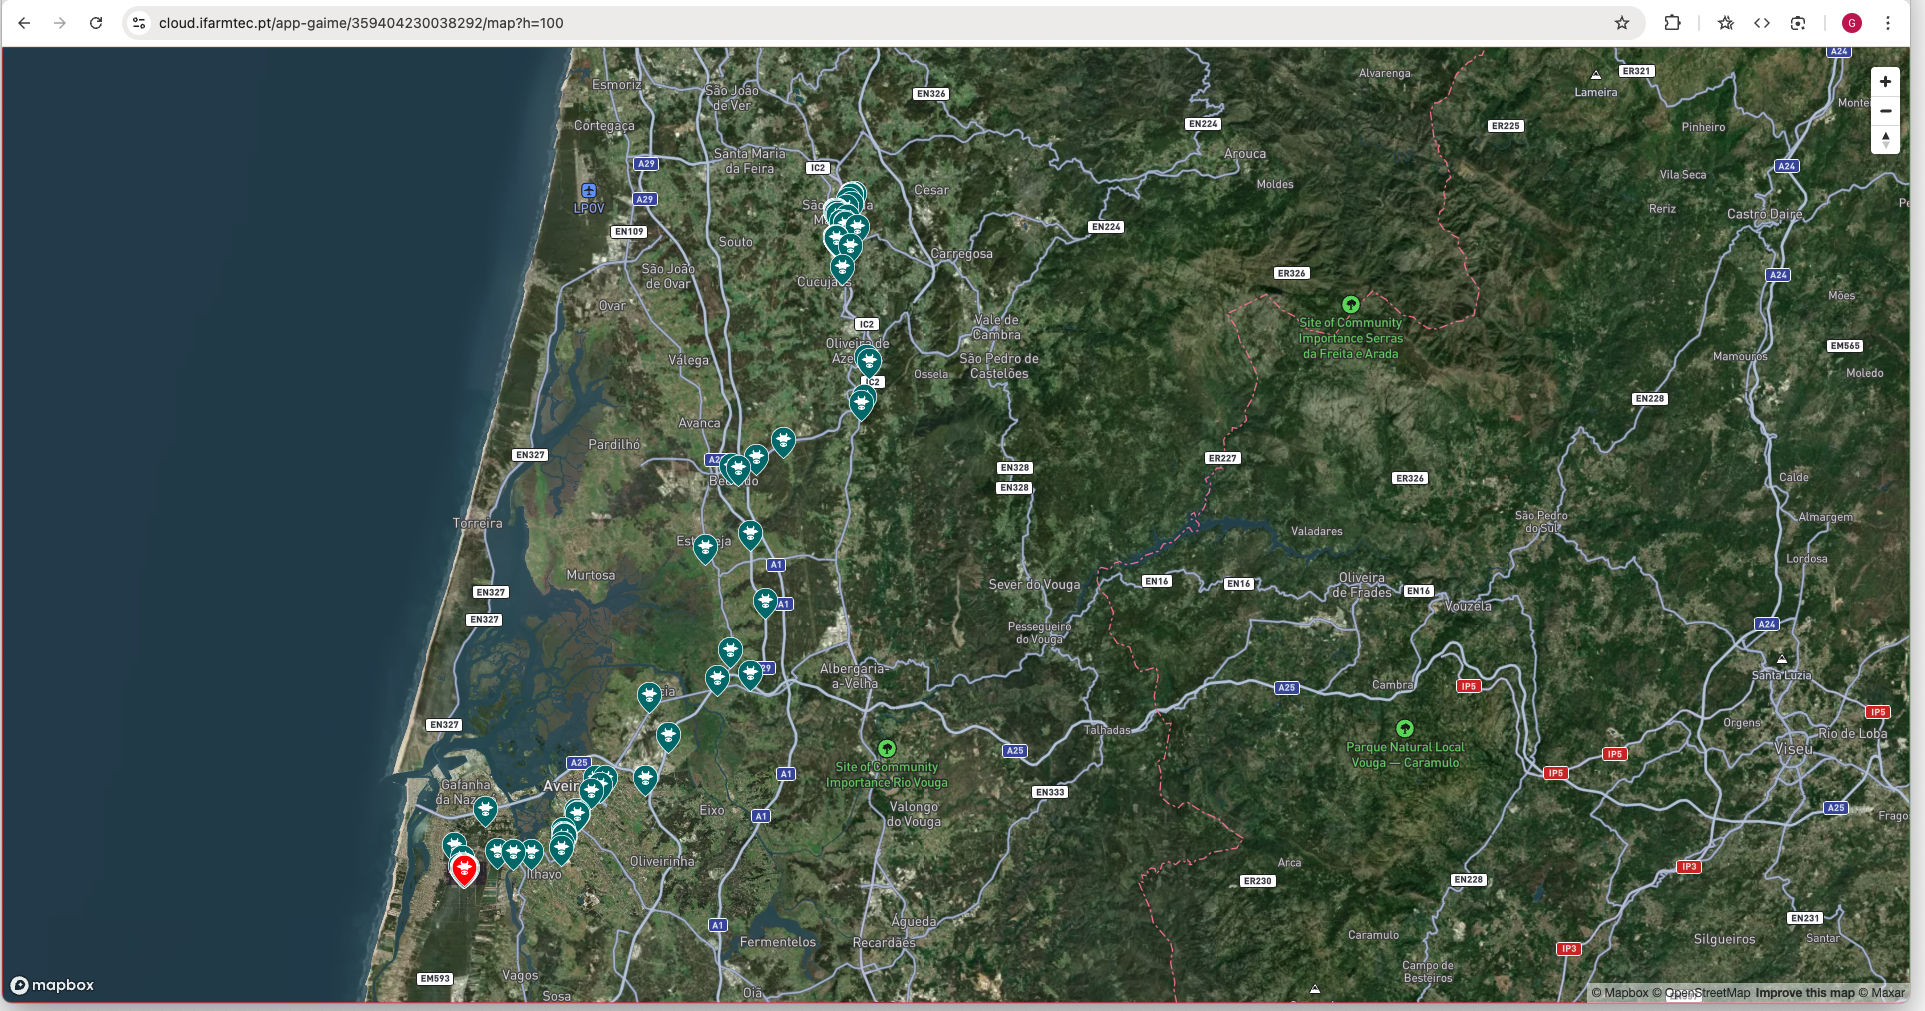
\includegraphics[width=\textwidth]{figs/mapbox.png}
    \caption[mapbox]{Mapbox}
    \label{fig:mapbox}
\end{figure}

\subsection{APIs de visualização gráfica}

\clearpage
\section{Interface gráfica}\label{sec:frontend}
    Nesta fase serão abordados com detalhes todo o trabalho realizado no \textit{frontend}/interface gráfica da aplicação. Problemas encontra

\subsection{Página de reset-pass}